\section{Results}

\subsection{Correlation and Regession Results to find Relevant Variables}
WRITE SOMETHING ABOUT USING REGRESSIONS TO SELECT VARIABLES 


\subsection{Exploratory Data Analysis}
After using correlation and regression to select features related to repayment, we were able to perform some exploratory data analysis. 

\begin{figure}
  \caption{Scatter Plot of Completion Rate vs. 3 Year Repayment Rate}
  \centering
  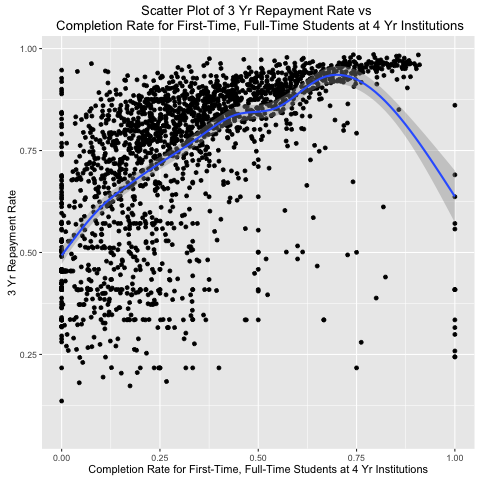
\includegraphics[width=0.6\textwidth]{../images/eda/complrt_rpy3yr_scatter.png}
  \centering
  \newline
  
  \raggedright
From the graph, we can see that schools with repayment rates below 75\% tend to have completion rates below 50\%. There is also a very steep trend for completion rate for repayment rates above 75\%. 
\end{figure}
 


\begin{figure}
  \caption{Scatter Plot of Different Tuition Types on 3 Year Repayment Rate}
  \centering
  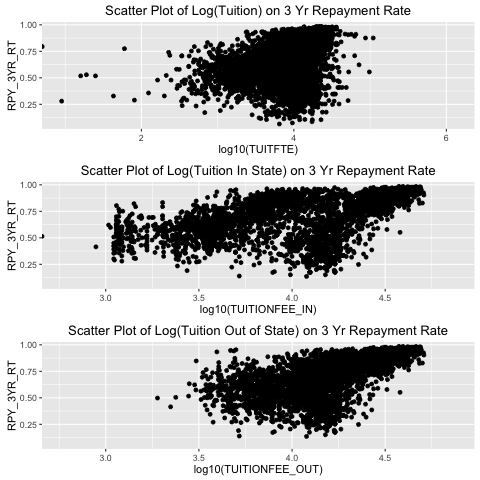
\includegraphics[width=0.6\textwidth]{../images/eda/rpy3yr_tuition_scatter.png}
  \centering
  \newline
  
  \raggedright
This figure displays three different scatterplots of Tuition fee vs Repayment Rate. In the data set, there are three different information of Tuition fee under cost category. First graph is a Net tuition revenue per full-time equivalent student vs repayment rate. Second graph is a In-stat tuition and fee vs repayment rate and last one is out-of-state tuition and fees vs repayment rate. There is highest correlation between out-of-state vs repayment rate.
\end{figure}


\begin{figure}
  \caption{Scatter Plot of 3 Year Repayment Rates on Type of Institution}
  \centering
  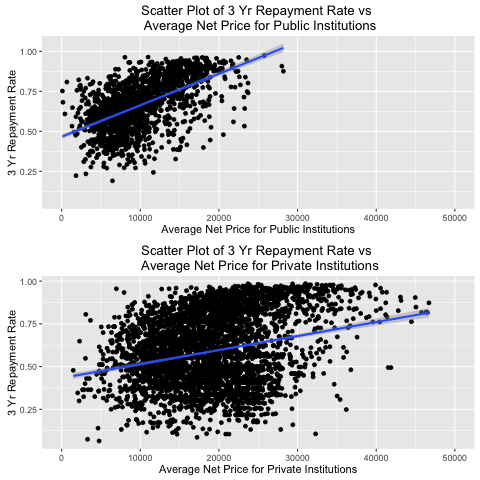
\includegraphics[width=0.6\textwidth]{../images/eda/netprice_pub_priv_rpy3yr_scatter}
  \centering
  \newline
  
  \raggedright
The figure aboce is a scatterplot of 3 Year Repayment Rate vs average net price for public institutions and below, it has a scatterplot of 3 Year Repayment Rate vs average net price for private instutitions. It shows higher slope for public institution but for both graph, it shows weak relationship between the average net price and repayment rate. 
\end{figure}


\begin{figure}
  \caption{Scatter Plot of Repayment Rates on Type of Institution}
  \centering
  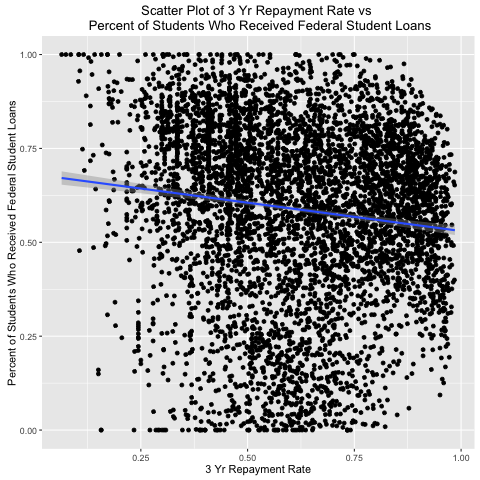
\includegraphics[width=0.6\textwidth]{../images/eda/pctfloan_rpy3yr_scatter}
  \centering
  \newline
  
  \raggedright
The figure aboce is a scatterplot of 3 Year Repayment Rate vs percent of students who received federal student loans. By looking the graph, it shows that there is weak relationship between percent of students who recieved federal student loans and 3yr repayment rate.
\end{figure}


\begin{figure}
  \caption{Barplot of Mean 3 Year Repayment Rate on REGION Levels}
  \centering
  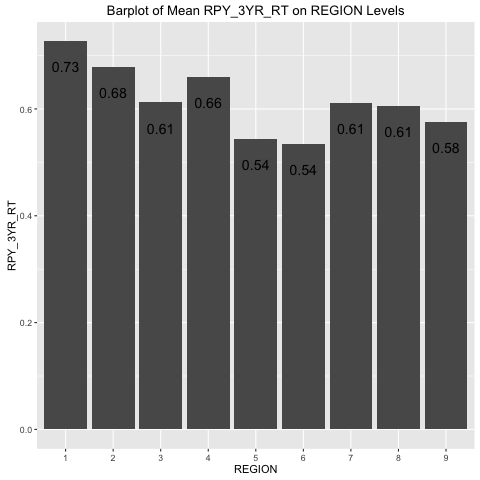
\includegraphics[width=0.6\textwidth]{../images/eda/rpy_region_barplot.png}
  \centering
  \newline
  
  \raggedright
This figure displays a barplot of average value of 3 Year Repayment Rate for each region. 3 Year Repayment Rate is defined as a fraction of repayment cohort who are not in default, and with loan balances that have declined three years since entering repayment, excluding enrolled and military deferment from calculation. (rolling averages) and each university is divided into 9 regions: 0	U.S. Service Schools, 1New England (CT, ME, MA, NH, RI, VT), 2	Mid East (DE, DC, MD, NJ, NY, PA), 3	Great Lakes (IL, IN, MI, OH, WI),4	Plains (IA, KS, MN, MO, NE, ND, SD), 5	Southeast (AL, AR, FL, GA, KY, LA, MS, NC, SC, TN, VA, WV), 6	Southwest (AZ, NM, OK, TX), 7	Rocky Mountains (CO, ID, MT, UT, WY), 8	Far West (AK, CA, HI, NV, OR, WA), 9	Outlying Areas (AS, FM, GU, MH, MP, PR, PW, VI). Our graph is not showing region 0 because there is one university that is under region 0 and it did not have a value for 3 Year Repayment Rate On barplot it shows that region 1 and 2 have highest repayment rate(0.73 and 0.68, respectively) and region 5 and 6 have lowest repayment rate (0.54)
\end{figure}


\begin{figure}
  \centering
  \caption{Barplot of Mean 3 Year Repayment Rate on Control Levels and Distributions of 3 Year Repayment Rate for Control Level}
  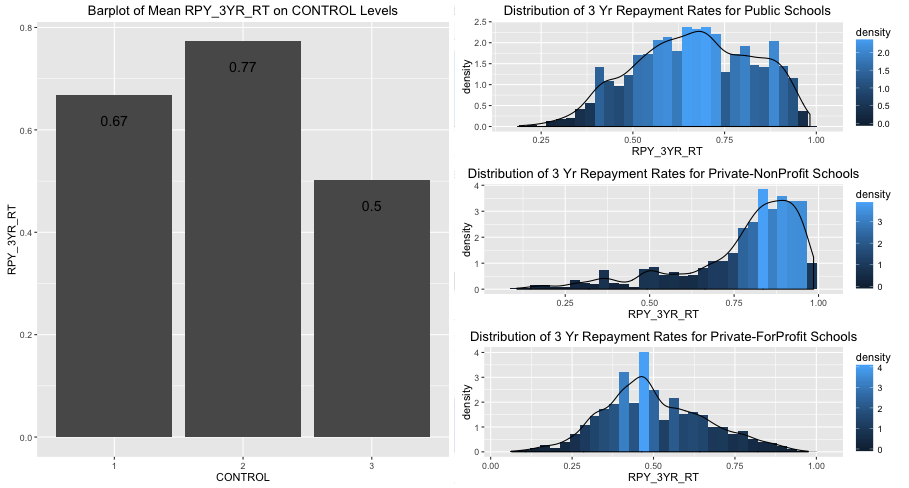
\includegraphics[width=0.6\textwidth]{../images/eda/rpy3yr_control_barplot_histogram.png}
  \centering
  \newline
  
  \raggedright
This figure displays a barplot that shows average value of 3 Year Repayment Rate for each school type. Under Control column, each school is divided into three categories: 1 = Public, 2 = Private nonprofit, 3 = Private for-profit. It shows that Private for nonprofit universities has highest average repayment rate with 0.77. On the right side, histogram helps for the better understanding of barplot. The visualizations on the right shows density graph and histogram of each institution's repayment rate.
\end{figure}


\begin{figure}
  \caption{Barplot of Mean 3 Year Repayment Rate on ICLEVEL Levels and Distributions of 3 Year Repayment Rate for each ICLEVEL Level}
  \centering
  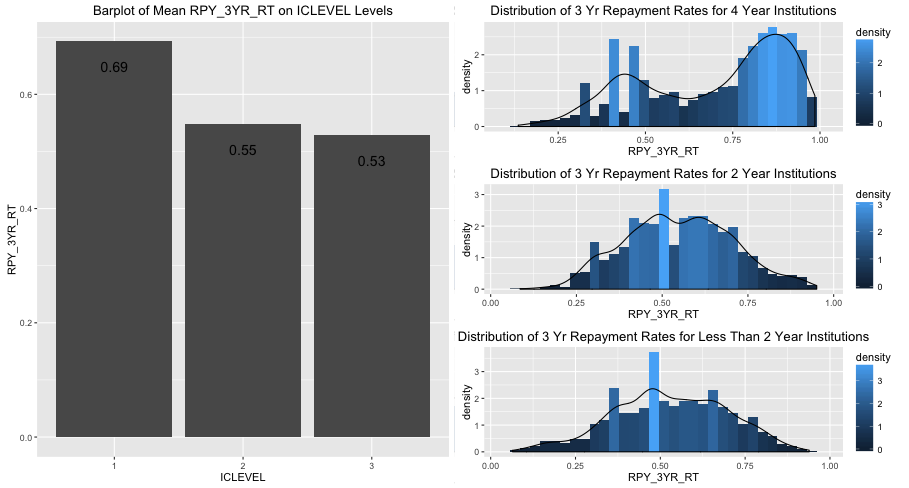
\includegraphics[width=0.6\textwidth]{../images/eda/iclevel_rpy3yr_barplot_histogram.png}
  \centering
  \newline
  
  \raggedright
This figure is a barplot that shows average value of 3 Year Repayment Rate for each level of institution. Uncer ICLEVEL, each school is divided into three categories: 1 = 4-year,2 = 2-year, 3 = Less-than-2-year. It shows that 4-year institution has the highest average repayment rate with 0.69. On the right side of the barplot, there is a histogram/desnity plot of each institution's repayment rate for detailed analysis.
\end{figure}

\begin{kframe}


{\ttfamily\noindent\bfseries\color{errorcolor}{\#\# Error in data.frame(rpy\_3yr\_regsum\$Coefficients, rpy3yr\_rr\_coef, rpy3yr\_lr\_coef, : arguments imply differing number of rows: 0, 8, 7}}

{\ttfamily\noindent\bfseries\color{errorcolor}{\#\# Error in colnames(coef.df) <- c("{}OLS"{}, "{}Ridge"{}, "{}Lasso"{}, "{}PCR"{}, "{}PLSR"{}): object 'coef.df' not found}}

{\ttfamily\noindent\bfseries\color{errorcolor}{\#\# Error in xtable(coef.df, caption = "{}Coefficients for each regression function"{}, : object 'coef.df' not found}}

{\ttfamily\noindent\bfseries\color{errorcolor}{\#\# Error in print(coef\_latex, comment = FALSE, table.placement = "{}H"{}, type = "{}latex"{}, : object 'coef\_latex' not found}}\end{kframe}

